Un wiki es una aplicación web que permite a los usuarios la adición, modificación o eliminación de contenido en colaboración con otros \cite{Wiki}. Dentro de las implementaciones de wiki existentes, el proyecto de enciclopedia Wikipedia es el más popular en Internet y una de las páginas web más grandes del mundo con más de 18 billones de visitas al mes y 30 millones de artículos en 287 idiomas \cite{Wikipedia}.
A diferencia de las enciclopedias tradicionales, Wikipedia permite a cualquier usuario registrado o no la edición del contenido de sus artículos. Ningún usuario es considerado el dueño de un artículo, y su contenido no es vetado ni aprobado por autoridad reconocida alguna. Es por ello que los editores deben ponerse de acuerdo sobre el contenido y estructura del artículo a través del consenso \cite{Wikipedia}.

Para facilitar la colaboración, todos los artículos de Wikipedia tienen asociado un historial de revisiones, que permite a los editores restaurar contenido perdido y deshacer cambios no deseados. El historial de revisiones, es una página que contiene una lista de las ediciones realizadas sobre un artículo, que incluyen la fecha y hora de cada edición, el nombre de usuario o IP del editor y un resumen de edición \cite{WikiHelp}.

Según Scalise \cite{Sca08}, los sistemas basados en MediaWiki, como Wikipedia, no explotan propiedades presentes en los datos de los historiales; en particular, la evolución de cada artículo, la comunidad de usuarios participantes y la frecuencia de los cambios. Además enfatiza que carecen de una visualización gráfica de los datos. Esto último ha sido el objeto de estudio de muchas investigaciones.

La literatura sobre visualizaciones de historiales de Wikipedia contiene en general visualizaciones que pueden clasificarse en dos grupos. El primero de ellos se enfoca en el estudio de la interacción de los editores de un artículo mediante visualizaciones de redes \cite{Suh07}, \cite{Kee12}, mientras que el segundo se centra en el estudio de la evolución de las propiedades de los artículos mediante su visualización en series temporales \cite{Vie04}, \cite{Wat07}, \cite{Nun08}. Estos trabajos han permitido analizar la dinámica y coordinación de los editores, como también la detección de patrones de actividad, conflicto y vandalismo. En general, han permitido alcanzar conclusiones importantes sobre el comportamiento de la comunidad colaborativa de Wikipedia.

Otro grupo de trabajos elaboró aplicaciones web cuya finalidad es monitorear el estatus del historial de un artículo. Entre esos están el WikiDashboard \cite{Suh08} y una herramienta estadística integrada en Wikipedia \cite{Aka}. A diferencia de las aplicaciones anteriores, que se enfocan en generar visualizaciones exploratorias de todo el historial, este grupo de aplicaciones se centró en crear un monitor de actividades recientes que mantuviera actualizados a los usuarios con el fin de mejorar la transparencia y responsabilidad social en artículos de Wikipedia. Ello se logra a través de visualizaciones que dan múltiples representaciones (líneas de tiempo, cromograma, listas de usuario, etc.) de la información reciente de manera resumida.

\section{History Flow}
Una de las primeras visualizaciones de historiales de Wikipedia fue History Flow \cite{Vie04}, que plantea una herramienta de análisis exploratorio de datos efectiva para revelar patrones sobre el comportamiento de una comunidad colaborativa como Wikipedia \Fig{fig:fig2}{}. El objetivo de History Flow es garantizar la visualización inmediata de tendencias generales del historial de revisiones preservando los detalles para una exploración más minuciosa.

\begin{figure}[htp]
  \centering
  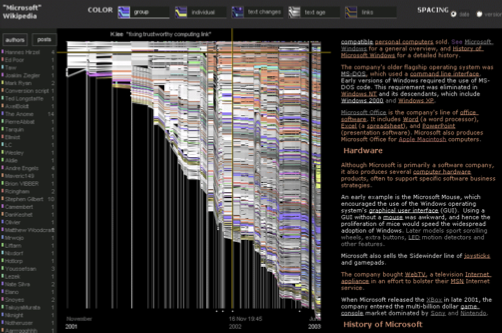
\includegraphics[width=0.75\textwidth]{fig2.png}
  \caption[Interfaz de usuario de la herramienta History Flow]{Interfaz de usuario de la herramienta History Flow explorando el artículo de Microsoft en Wikipedia. A la derecha se observa el contenido de la página, a la izquierda se despliega la lista de editores del artículo y en el panel central se muestra la visualización \cite[Fig. 3]{Vie04}.}
  \label{fig:fig2}
\end{figure}

Para explicar el método, se plantea el siguiente escenario. Tres autores (María, Susana y Andrés) colaboran en la redacción de un artículo. A cada colaborador se le asigna un color que lo va a representar en la visualización. En primer lugar, María crea el documento y añade una cantidad de texto. Esta versión es reflejada como una “línea de versión” vertical, de color negro y con una longitud proporcional a la longitud del texto \Fig{fig:fig1}{a}. En la siguiente versión, Susana agrega texto al final del documento sin modificar lo hecho por María. La línea de versión ahora mostrará una sección de color blanco (correspondiente a Susana) debajo de la sección de María. De esta forma, la línea de revisión aumenta su longitud en esta versión para reflejar el crecimiento del documento.

\begin{figure}[htp]
  \centering
  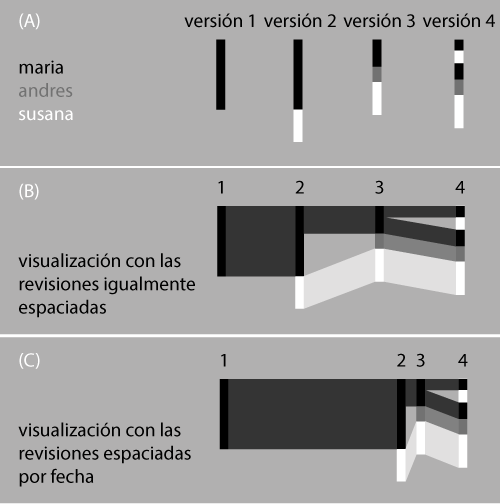
\includegraphics[width=0.6\textwidth]{fig1.png}
  \caption[Explicación del mecanismo de visualización History Flow]{Explicación del mecanismo de visualización History Flow \cite[Fig. 2]{Vie04}.}
  \label{fig:fig1}
\end{figure}

En la versión 3, Andrés elimina una porción del texto original de María e introduce una pequeña contribución entre los textos de María y Susana. Finalmente, en la versión 4 Susana agrega texto en el medio de lo que resta del contenido de María.

Con el fin de observar las relaciones entre las diferentes versiones, el diagrama de History Flow vincula la sección de texto que se ha mantenido igual entre versiones consecutivas. Esto se logra dibujando conexiones sombreadas entre segmentos correspondientes a líneas de versión adyacentes \Fig{fig:fig1}{b}. Los segmentos de texto que no tienen correspondencia en versiones adyacentes no se conectan y por ello el usuario observa el vacío en la visualización, destacando así claramente las inserciones y eliminaciones.

Una variante del History Flow emplea el espacio entre las líneas de revisión para reflejar el paso del tiempo. De esta forma, en lugar de utilizar el mismo espaciado entre líneas de revisión se coloca un espaciado proporcional a la diferencia entre fechas de revisiones sucesivas \Fig{fig:fig1}{c}. Esta variante tiene el beneficio de revelar los ritmos de colaboración entre autores.

\section{Chromogram}
El Cromograma es una técnica de visualización empleada por Wattenberg y Viegas \cite{Wat07} para investigar la distribución del tiempo de los participantes de la comunidad colaborativa de Wikipedia. Consiste esencialmente en una visualización exploratoria que hace una codificación cromática de largas secuencias textuales, produciendo una visualización densa en datos que puede contener la vasta historia de ediciones de un usuario en una pantalla \Fig{fig:fig8-9}{}. Esta visualización permitió la identificación de patrones de actividades reactivas y sistemáticas en la comunidad colaborativa de Wikipedia.

\begin{figure}[htp]
  \begin{subfigure}[b]{0.45\textwidth}
    \centering
    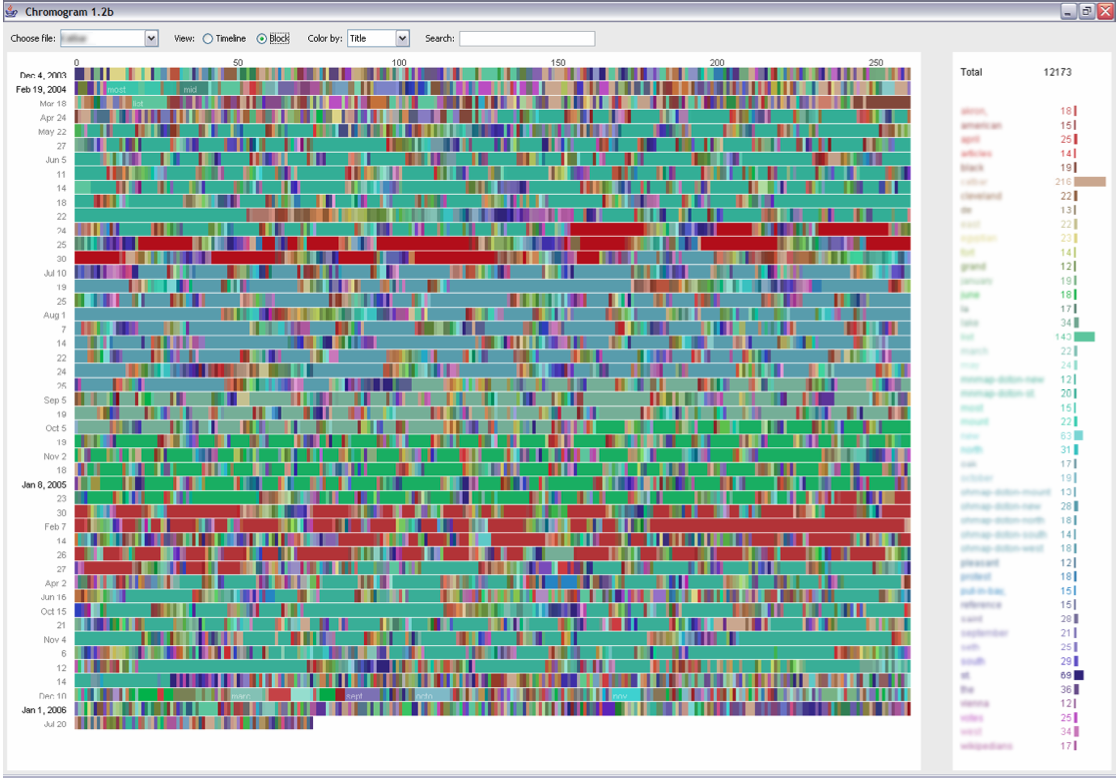
\includegraphics[width=\textwidth]{fig8.png}
    \caption[]{Vista de bloque \cite[Fig. 3]{Wat07}.}
    \label{fig:fig8}
  \end{subfigure}
  \hfill
  \begin{subfigure}[b]{0.45\textwidth}
    \centering
    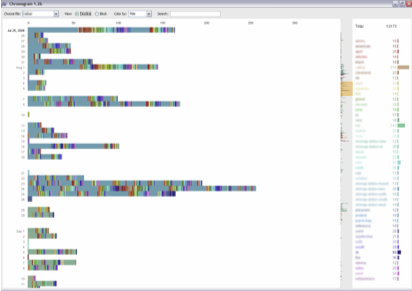
\includegraphics[width=\textwidth]{fig9.png}
    \caption[]{Vista en línea de tiempo \cite[Fig. 4]{Wat07}.}
    \label{fig:fig9}
  \end{subfigure}
  \caption[La aplicacieon Chromogram]{La aplicación Chromogram. Exploración de los cromogramas de los 509 administradores de Wikipedia para el momento del estudio.}
  \label{fig:fig8-9}
\end{figure}

El criterio de codificación toma las primeras tres letras para determinar el color de la representación. La primera letra determina el tono, la segunda la saturación y la tercera el brillo. Se restringe el rango de la saturación y el brillo de manera que el tono pueda percibirse fácilmente. Como caso especial, se codifican en escala de grises los títulos o comentarios que comienzan con un número. \Figlink{fig:fig6}{} muestra ejemplos de esta codificación usando palabras comunes encontradas en los comentarios de los usuarios de Wikipedia.

\begin{figure}[htp]
  \centering
  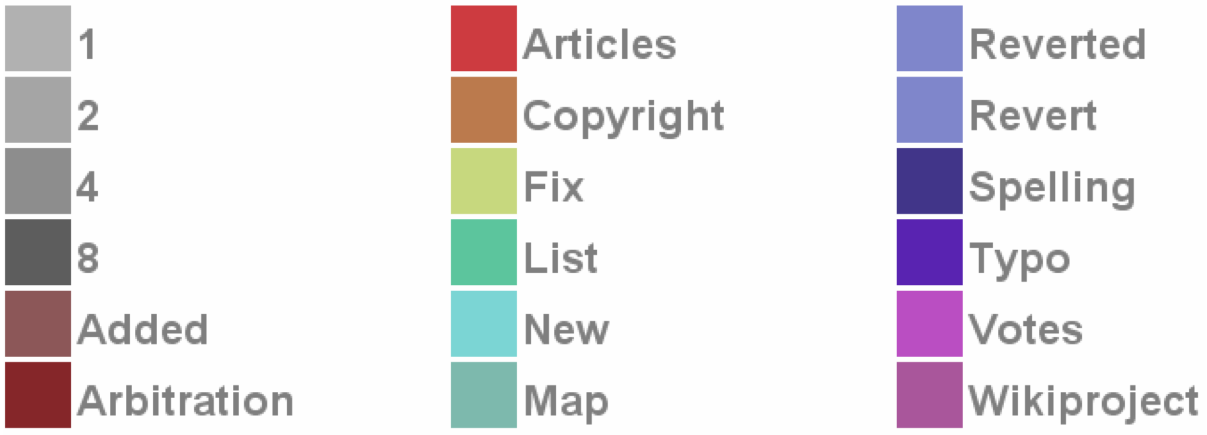
\includegraphics[width=0.6\textwidth]{fig6.png}
  \caption[Codificación de palabras a color]{Codificación de palabras a color \cite[Fig. 1]{Wat07}.}
  \label{fig:fig6}
\end{figure}

La técnica del Cromograma parte de esta codificación y permite visualizar una larga historia de revisión en una sola pantalla. Para explicarla, en primer lugar se muestra \figlink{fig:fig7}{a} una lista hipotética de revisiones. La visualización consiste entonces en tomar el texto del comentario de cada elemento de la lista, codificarlo y crear un histograma \Fig{fig:fig7}{b} donde cada fila corresponde a un día y contiene un rectángulo para cada revisión ordenada en el tiempo. \Figlink{fig:fig7}{c} muestra la variante de la visualización llamada “vista de bloque”, en la cual las revisiones se muestran de manera continua y consolidada ordenadas en el tiempo de izquierda a derecha y luego de arriba a abajo. Esta vista es más densa, pero oculta los ritmos temporales de las revisiones.

\begin{figure}[htp]
  \centering
  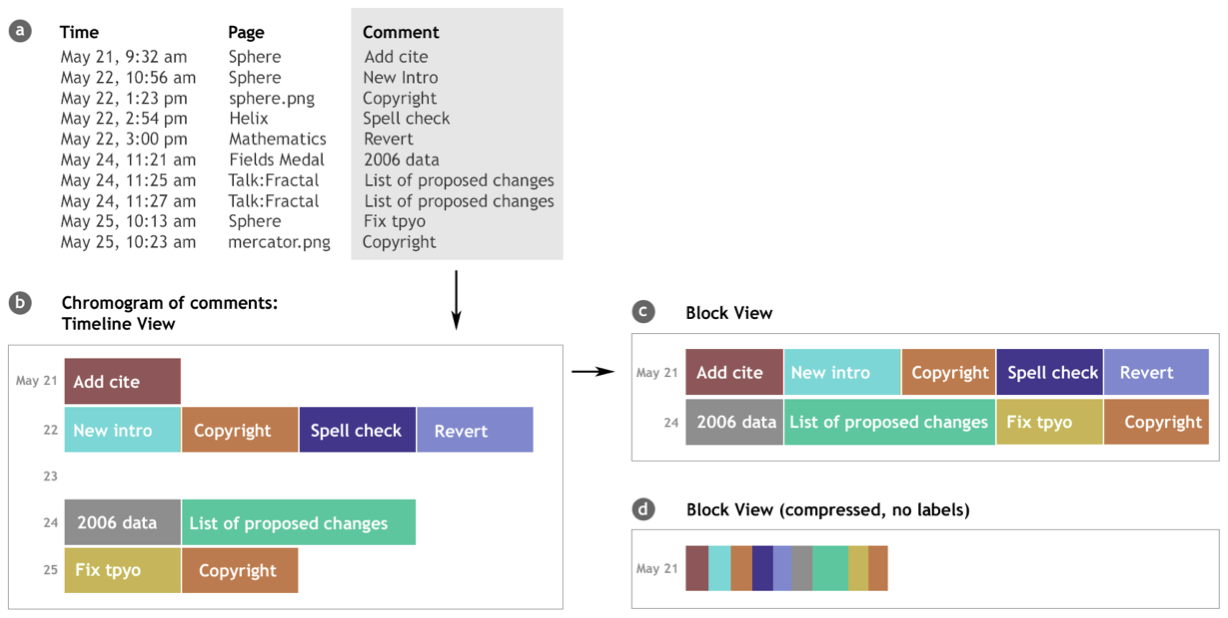
\includegraphics[width=0.95\textwidth]{fig7.png}
  \caption[Creando un Cronograma]{Creando un Cromograma \cite[Fig. 2]{Wat07}.}
  \label{fig:fig7}
\end{figure}

\section{WikiChanges}
Es una aplicación web diseñada con la finalidad de estudiar la correlación entre la popularidad de un tema y el perfil de actualización \cite{Nun08}. Esto se logra mediante una visualización que grafica sobre una línea de tiempo el número de revisiones que sufre un artículo, acompañado de un resumen de revisiones que crea una nube términos que ayuda a determinar los eventos asociados a picos de actividad.

Según el autor, el perfil de actualización es “la distribución de revisiones en el tiempo hecha sobre un artículo en un sistema de wiki”. Para construir el perfil de actualización de un artículo de Wikipedia, se extrae la fecha de cada revisión, se cuenta el número de revisiones por período (día, mes o año) y se produce una serie de tiempo.
\Figlink{fig:fig10}{}, muestra el perfil de actualización del artículo sobre Steve Fossett. Se puede observar un pico de actividad en Septiembre del 2007, fecha en la cual fue reportado desaparecido durante un vuelo, y luego otro en Febrero del 2008 cuando fue declarado muerto. Dado que en este caso se conocen de antemano los eventos asociados al artículo, es fácil predecir y entender los picos de actividad. Sin embargo, cuando estos eventos asociados no se conocen, la visualización por sí sola no permite descubrir las posibles causas de los picos de actividad. Como solución a esta limitante, se planteó la construcción automática de “resúmenes”.

\begin{figure}[htp]
  \centering
  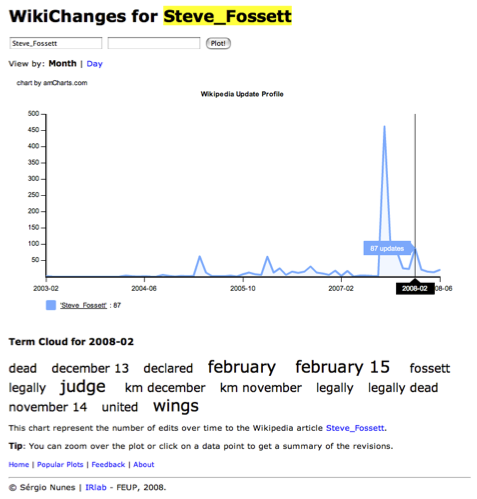
\includegraphics[width=0.75\textwidth]{fig10.png}
  \caption[Sistema WikiChanges mostrando la historia de revisiones para el artículo de Steve Fossett]{Sistema WikiChanges mostrando la historia de revisiones para el artículo de Steve Fossett \cite[Fig. 3]{Nun08}.}
  \label{fig:fig10}
\end{figure}

Estos resúmenes se construyen para un período dado usando un enfoque basado en los términos insertados entre revisiones. Sólo se considera la versión más antigua y la más reciente del documento analizado en el período definido. De cada versión se prepara un conjunto de términos acompañados de su frecuencia. Los términos pueden ser una palabra (unigrams) o  la ocurrencia de dos palabras consecutivas (bigrams). Sustrayendo la frecuencia de los términos en la versión más antigua de la más reciente obtenemos el conjunto que formará la nube de términos para el período determinado. Cada término es ponderado usando su frecuencia resultante, como se muestra \figlink{fig:fig10}{}.

\section{Revert Graph}
En este trabajo se describió un modelo para identificar patrones de conflicto en artículos de Wikipedia \cite{Suh07}. El modelo se basa en el historial de ediciones de usuarios y las relaciones entre sus ediciones, especialmente aquellas que eliminan ediciones previas; conocidas como “reversiones” o “reverts”. Revert Graph es una herramienta que utiliza grafos de nodos para visualizar patrones de conflicto generales entre grupos de usuarios.

Se plantean dos métodos para identificar “reversiones” en Wikipedia. El primero se basa en calcular un identificador único para cada revisión en un artículo usando un esquema de hashing MD5. Se usa la función de MD5 para generar una pequeña huella digital de cada revisión, la cual permite una rápida comparación entre todos los artículos. El segundo método permite capturar las “reversiones” parciales usando las etiquetas “revert” y “rv” en los comentarios del editor en cada revisión.

Inicialmente, la herramienta carga un grupo de usuarios participando en la edición de un artículo como un grafo de nodos uniformemente distribuido. La simulación ejecuta un algoritmo de disposición que simula la dinámica social que resulta del modelo de conflicto de usuarios. Este algoritmo asigna fuerzas tal que los bordes (que representan relaciones de reversión) funcionan como resortes, mientras que los usuarios son representados como partículas con campos gravitacionales. A medida que la simulación progresa, las fuerzas del grafo se estabilizan y las estructuras sociales entre usuarios empiezan a emerger, como se muestra \figlink{fig:fig11}{}. El tamaño del nodo es proporcional al número de reversiones o revisiones. Los nodos son codificados con color basándose en el estatus de registro de los usuarios. Un administrador se colorea como un nodo verde, un usuario registrado normal como uno gris y uno no registrado como uno blanco.

\begin{figure}[htp]
  \centering
  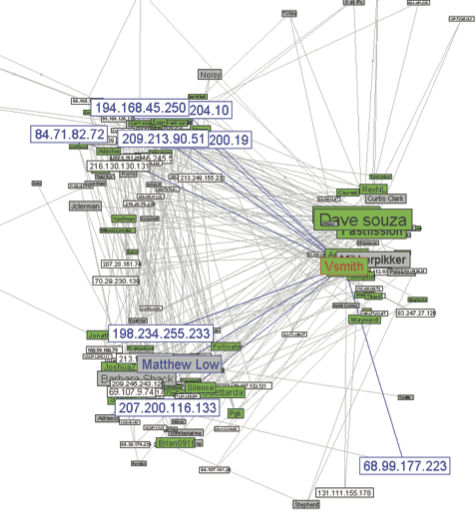
\includegraphics[width=0.75\textwidth]{fig11.png}
  \caption[Visualización Revert Graph del artículo de Charles Darwin]{Visualización Revert Graph del artículo de Charles Darwin \cite[Fig. 1]{Suh07}.}
  \label{fig:fig11}
\end{figure}

\section{Estructuras y Dinámicas de las Colaboraciones en Wikipedia en Eventos Recientes}
Este trabajo estudia la dinámica de coordinación de los editores de Wikipedia sobre dos categorías de artículos: aquellos sobre eventos recientes y aquellos sobre acontecimientos históricos \cite{Kee12}. Los resultados mostraron que las estructuras y dinámicas son distintas entre artículos para estas dos categorías y que tienen implicaciones en cómo los sistemas de inteligencia colectiva pueden apalancarse para procesar y dar sentido a información compleja.

La visualización empleada en este estudio usa una perspectiva de análisis de red. Este enfoque se basa en la construcción de una “trayectoria de artículo”, que es la secuencia temporal de las revisiones contenidas en el historial. Los nodos en la trayectoria son los autores, mientras que las conexiones entre nodos representan las revisiones que transicionan el artículo de la revisión de un autor a la del siguiente. Un lazo ocurre cuando un solo editor guarda múltiples revisiones a lo largo del historial de un artículo \Fig{fig:fig12}{}. Una cadena aparece cuando editores subsecuentes hacen revisiones únicas sin contribuir nuevamente en el artículo \Fig{fig:fig13}{}. En general, esta técnica captura una vista estructural de la historia de revisiones que permite visualizar y analizar relaciones complejas entre editores y las versiones de un artículo.

\begin{figure}[htp]
  \begin{subfigure}[b]{0.45\textwidth}
    \centering
    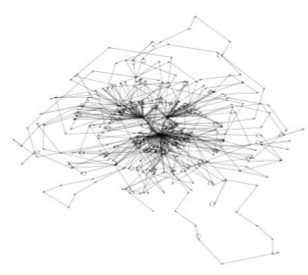
\includegraphics[width=\textwidth]{fig12.png}
    \caption[]{Adam Air Vuelo 574 (Artículo de última hora) \cite[Fig. 2a]{Kee12}.}
    \label{fig:fig12}
  \end{subfigure}
  \hfill
  \begin{subfigure}[b]{0.45\textwidth}
    \centering
    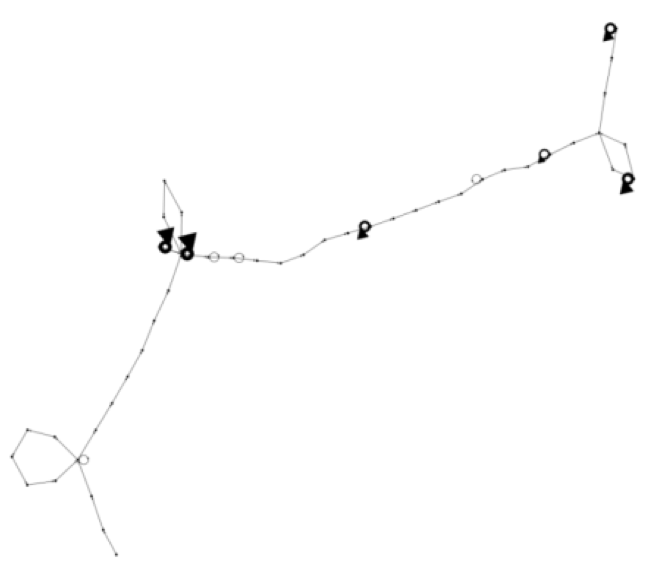
\includegraphics[width=\textwidth]{fig13.png}
    \caption[]{Lufthansa Vuelo 2904 (Artículo sobre acontecimiento histórico) \cite[Fig. 2d]{Kee12}.}
    \label{fig:fig13}
  \end{subfigure}
  \caption[Visualizaciones de dos artículos tomados de la lista de accidentes de aviones comerciales de Wikipedia]{Visualizaciones de dos artículos tomados de la lista de accidentes de aviones comerciales de Wikipedia.}
\end{figure}

\section{Visualización de Propiedades de Historiales de Artículos de Wikis Mediante un Enfoque de Ingeniería Dirigida por Modelos}
En este trabajo se describe un enfoque dirigido por modelos para el procesamiento de los historiales de artículos de un sistema Wiki basado en MediaWiki \cite{Sca08}. En él se describe cómo se pueden calcular propiedades alternas a las disponibles, así como la generación de reportes y visualizaciones gráficas de la información.

El proceso planteado consiste en definir un metamodelo del dominio \Fig{fig:fig14}{} el cual es empleado para generar un modelo que describa los historiales. El modelo es luego usado para desarrollar transformaciones que calculen propiedades sobre los datos. Se definen tres tipos de propiedades: generales, con clasificador y específicas. Las generales son propiedades numéricas (enteras o reales) calculadas para un artículo. Las propiedades con clasificador son aquellas similares a las generales, pero que agrupan o discriminan por una condición denominada clasificador. Las propiedades específicas son aquellas orientadas a visualizaciones particulares o reportes de los datos gestionados por el Wiki. Se cita como ejemplo de propiedad específica la calculada para la generación del gráfico History Flow.

\begin{figure}[htp]
  \centering
  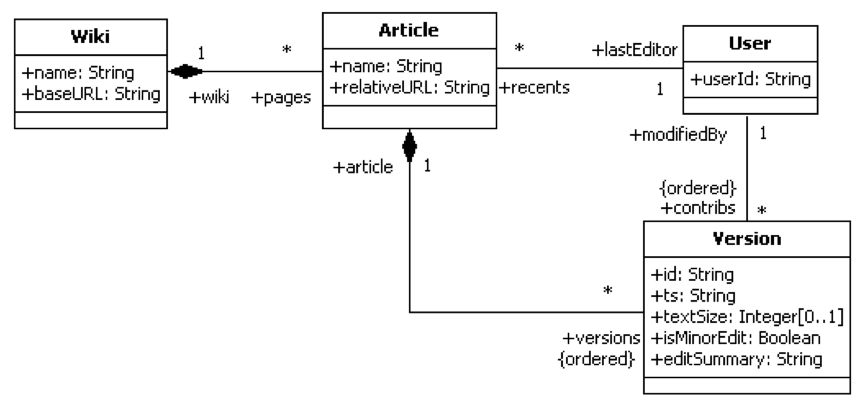
\includegraphics[width=0.75\textwidth]{fig14.png}
  \caption[Metamodelo de implementación de los artículos de un Wiki y su historial]{Metamodelo de implementación de los artículos de un Wiki y su historial \cite[Fig. 2]{Sca08}.}
  \label{fig:fig14}
\end{figure}

Por último, se generan reportes o representaciones gráficas con las propiedades (métricas) calculadas. En el trabajo se hacen las siguientes recomendaciones en ese sentido:

\begin{itemize}
  \item Si se desean comparar las propiedades generales entre distintos artículos del Wiki, resultan apropiado los reportes mediante tablas o diagramas de barras.
  \item Si la visualización corresponde a propiedades con clasificador, entonces se recomiendan reportes textuales en forma de tablas y diagramas de torta (pie charts) para visualizar porcentajes.
\end{itemize}

Para la visualización de propiedades generales y con clasificador, se siguió un enfoque en el cual se escoge el metamodelo de visualización apropiado y luego se escribe la transformación para generar la instancia con los datos del historial del wiki. Por último se importan los resultados hacia cualquier herramienta de visualización utilizando una transformación.

En el ámbito de las propiedades específicas, se desarrolló una adaptación del gráfico History Flow, denominada History Graph. La estrategia usada para implementar esta visualización fue definir el metamodelo \Fig{fig:fig15}{} y luego escribir una transformación a partir de los datos extraídos de MediaWiki. En general, las propiedades específicas no siguen ningún patrón. A causa de ello, es necesario definir un metamodelo particular para cada propiedad.

\begin{figure}[htp]
  \centering
  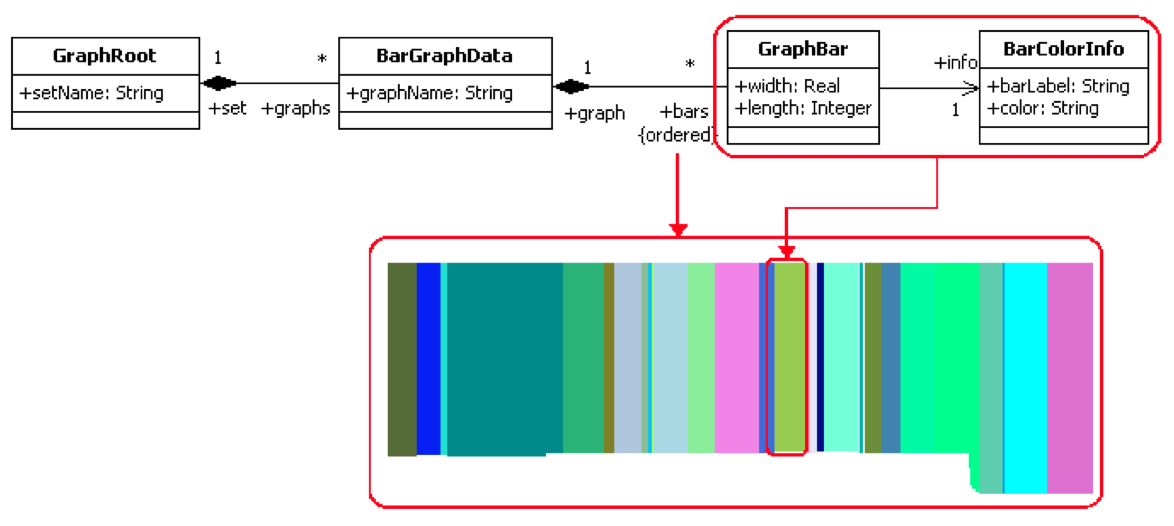
\includegraphics[width=0.75\textwidth]{fig15.png}
  \caption[Metamodelo de History Graph y relación con una visualización]{Metamodelo de History Graph y relación con una visualización \cite[Fig. 6]{Sca08}.}
  \label{fig:fig15}
\end{figure}

El trabajo concluye que la propuesta planteada permite recuperar información del web siguiendo un enfoque flexible, que disminuye las dependencias de los programas con respecto a los aspectos de formato y separa el cálculo de las propiedades de su posterior visualización, lo cual trae el beneficio de permitir que una misma propiedad pueda ser visualizada de diferentes formas.

\section{Métodos y Técnicas para el Cálculo y Visualización de Métricas de Historiales de Artículos Wiki}
En su trabajo, D’Apuzzo y Worwa implementan una aplicación (Web Scraper) que permite la recuperación del historial de los artículos de cualquier Wiki basado en MediaWiki, para luego calcular métricas y propiedades de interés asociadas a dicha información \cite{Dap12}. El trabajo halla su motivación en la carencia de herramientas gráficas para el análisis y visualización de propiedades de los historiales que permitan observar su evolución en el tiempo.

Un Web Scraper es un programa automatizado que se encarga de visitar de manera sistematizada un conjunto de URLs con el fin de obtener información y/o realizar actividades de rutina o mantenimiento. En este caso, se implementó un Web Scraper para la extracción de historiales de sistemas basados en MediaWiki con las siguientes políticas de selección, revisita y cortesía:

\begin{description}
  \item[Selección:] las URL a visitar son provistas por el usuario final; una a la vez, o por lote mediante un archivo de texto en el cual se especifica una URL por línea. Las URL suministradas son sometidas a un proceso de normalización.
  \item[Revisita:] la política de revisita se basa en un sistema de prioridades. Una URL recién almacenada tiene una prioridad de 0.5. Luego de visitada y de haber extraído la información, la prioridad se actualiza con el valor 0. Esta probabilidad irá aumentando en el tiempo de acuerdo a la formula:

\begin{equation}
  1-\frac{T_{0}}{T_{i}}
\end{equation}

donde To es la marca de tiempo (timestamp) de la última fecha de actualización de la URL (por defecto 0) y Ti es la marca de tiempo del momento en que se está calculando la prioridad de revisita.
  \item[Cortesía:] Se espera un tiempo mínimo de 10 segundos entre peticiones al servidor.
\end{description}

Como se muestra \figlink{fig:fig16}{}, la arquitectura del Web Scraper incluye dos módulos de soporte: una herramienta de URL y un demonio de prioridades. La herramienta de URL es una pequeña aplicación que recibe como parámetro una URL, la normaliza y la agrega al sistema. El demonio de prioridades se encarga de la actualización del valor de prioridad de las URL almacenadas en la base de datos usando la fórmula establecida en la política de revisita.

\begin{figure}[htp]
  \centering
  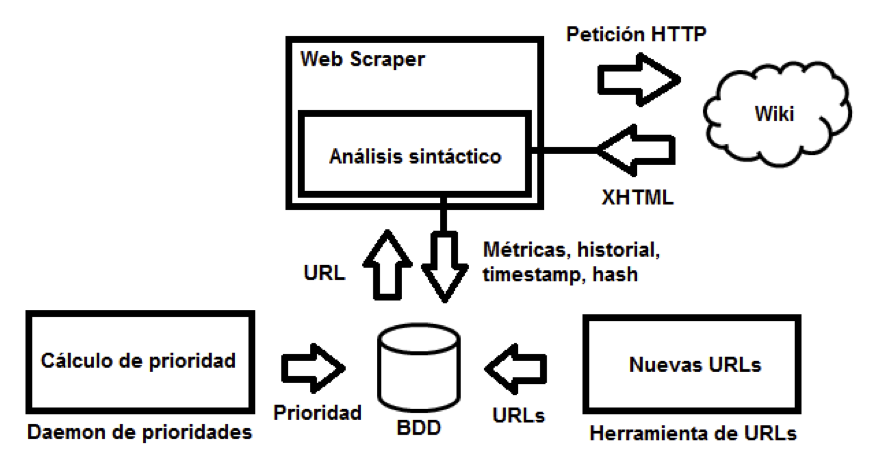
\includegraphics[width=0.75\textwidth]{fig16.png}
  \caption[Arquitectura del sistema WikiMetrics-UCV]{Arquitectura del sistema WikiMetrics-UCV \cite[Fig. 3.1]{Dap12}.}
  \label{fig:fig16}
\end{figure}

El funcionamiento del Web Scraper sucede de la siguiente manera. Dado el pool de semillas almacenadas en la base de datos por la herramienta de URLs, el Web Scraper selecciona la URL a visitar y se descarga el documento HTML, que luego pasa por un proceso de análisis sintáctico mediante el cual se extrae toda la información especificada por el usuario usando expresiones XPath. Está información es luego normalizada y almacenada en la base de datos.

La aplicación se implementó en lenguaje Python en combinación con una base de datos NoSQL manejada con MongoDB. Dicho proyecto se encuentra hospedado en la siguiente dirección de GitHub \footnote{\url{https://github.com/bworwa/wiki_metrics_ucv}}.
